\documentclass[10pt,ignorenonframetext,,aspectratio=149]{beamer}
\setbeamertemplate{caption}[numbered]
\setbeamertemplate{caption label separator}{: }
\setbeamercolor{caption name}{fg=normal text.fg}
\usepackage{lmodern}
\usepackage{amssymb,amsmath}
\usepackage{ifxetex,ifluatex}
\usepackage{fixltx2e} % provides \textsubscript
\ifnum 0\ifxetex 1\fi\ifluatex 1\fi=0 % if pdftex
  \usepackage[T1]{fontenc}
  \usepackage[utf8]{inputenc}
\else % if luatex or xelatex
  \ifxetex
    \usepackage{mathspec}
  \else
    \usepackage{fontspec}
  \fi
  \defaultfontfeatures{Ligatures=TeX,Scale=MatchLowercase}
  \newcommand{\euro}{€}
\fi
% use upquote if available, for straight quotes in verbatim environments
\IfFileExists{upquote.sty}{\usepackage{upquote}}{}
% use microtype if available
\IfFileExists{microtype.sty}{%
\usepackage{microtype}
\UseMicrotypeSet[protrusion]{basicmath} % disable protrusion for tt fonts
}{}
\usepackage{color}
\usepackage{fancyvrb}
\newcommand{\VerbBar}{|}
\newcommand{\VERB}{\Verb[commandchars=\\\{\}]}
\DefineVerbatimEnvironment{Highlighting}{Verbatim}{commandchars=\\\{\}}
% Add ',fontsize=\small' for more characters per line
\usepackage{framed}
\definecolor{shadecolor}{RGB}{248,248,248}
\newenvironment{Shaded}{\begin{snugshade}}{\end{snugshade}}
\newcommand{\AlertTok}[1]{\textcolor[rgb]{0.94,0.16,0.16}{#1}}
\newcommand{\AnnotationTok}[1]{\textcolor[rgb]{0.56,0.35,0.01}{\textbf{\textit{#1}}}}
\newcommand{\AttributeTok}[1]{\textcolor[rgb]{0.77,0.63,0.00}{#1}}
\newcommand{\BaseNTok}[1]{\textcolor[rgb]{0.00,0.00,0.81}{#1}}
\newcommand{\BuiltInTok}[1]{#1}
\newcommand{\CharTok}[1]{\textcolor[rgb]{0.31,0.60,0.02}{#1}}
\newcommand{\CommentTok}[1]{\textcolor[rgb]{0.56,0.35,0.01}{\textit{#1}}}
\newcommand{\CommentVarTok}[1]{\textcolor[rgb]{0.56,0.35,0.01}{\textbf{\textit{#1}}}}
\newcommand{\ConstantTok}[1]{\textcolor[rgb]{0.00,0.00,0.00}{#1}}
\newcommand{\ControlFlowTok}[1]{\textcolor[rgb]{0.13,0.29,0.53}{\textbf{#1}}}
\newcommand{\DataTypeTok}[1]{\textcolor[rgb]{0.13,0.29,0.53}{#1}}
\newcommand{\DecValTok}[1]{\textcolor[rgb]{0.00,0.00,0.81}{#1}}
\newcommand{\DocumentationTok}[1]{\textcolor[rgb]{0.56,0.35,0.01}{\textbf{\textit{#1}}}}
\newcommand{\ErrorTok}[1]{\textcolor[rgb]{0.64,0.00,0.00}{\textbf{#1}}}
\newcommand{\ExtensionTok}[1]{#1}
\newcommand{\FloatTok}[1]{\textcolor[rgb]{0.00,0.00,0.81}{#1}}
\newcommand{\FunctionTok}[1]{\textcolor[rgb]{0.00,0.00,0.00}{#1}}
\newcommand{\ImportTok}[1]{#1}
\newcommand{\InformationTok}[1]{\textcolor[rgb]{0.56,0.35,0.01}{\textbf{\textit{#1}}}}
\newcommand{\KeywordTok}[1]{\textcolor[rgb]{0.13,0.29,0.53}{\textbf{#1}}}
\newcommand{\NormalTok}[1]{#1}
\newcommand{\OperatorTok}[1]{\textcolor[rgb]{0.81,0.36,0.00}{\textbf{#1}}}
\newcommand{\OtherTok}[1]{\textcolor[rgb]{0.56,0.35,0.01}{#1}}
\newcommand{\PreprocessorTok}[1]{\textcolor[rgb]{0.56,0.35,0.01}{\textit{#1}}}
\newcommand{\RegionMarkerTok}[1]{#1}
\newcommand{\SpecialCharTok}[1]{\textcolor[rgb]{0.00,0.00,0.00}{#1}}
\newcommand{\SpecialStringTok}[1]{\textcolor[rgb]{0.31,0.60,0.02}{#1}}
\newcommand{\StringTok}[1]{\textcolor[rgb]{0.31,0.60,0.02}{#1}}
\newcommand{\VariableTok}[1]{\textcolor[rgb]{0.00,0.00,0.00}{#1}}
\newcommand{\VerbatimStringTok}[1]{\textcolor[rgb]{0.31,0.60,0.02}{#1}}
\newcommand{\WarningTok}[1]{\textcolor[rgb]{0.56,0.35,0.01}{\textbf{\textit{#1}}}}
\usepackage{graphicx,grffile}
\makeatletter
\def\maxwidth{\ifdim\Gin@nat@width>\linewidth\linewidth\else\Gin@nat@width\fi}
\def\maxheight{\ifdim\Gin@nat@height>\textheight0.8\textheight\else\Gin@nat@height\fi}
\makeatother
% Scale images if necessary, so that they will not overflow the page
% margins by default, and it is still possible to overwrite the defaults
% using explicit options in \includegraphics[width, height, ...]{}
\setkeys{Gin}{width=\maxwidth,height=\maxheight,keepaspectratio}

% Comment these out if you don't want a slide with just the
% part/section/subsection/subsubsection title:
\AtBeginPart{
  \let\insertpartnumber\relax
  \let\partname\relax
  \frame{\partpage}
}
\AtBeginSection{
  \let\insertsectionnumber\relax
  \let\sectionname\relax
  \frame{\sectionpage}
}
\AtBeginSubsection{
  \let\insertsubsectionnumber\relax
  \let\subsectionname\relax
  \frame{\subsectionpage}
}

\setlength{\emergencystretch}{3em}  % prevent overfull lines
\providecommand{\tightlist}{%
  \setlength{\itemsep}{0pt}\setlength{\parskip}{0pt}}
\setcounter{secnumdepth}{0}

\title{EST-46114 Métodos Multivariados y Datos Categóricos}
\subtitle{Sesion 03 - Inferencia en la Distribucion Gaussiana Multivariada - Parte
2}
\author{Juan Carlos Martinez-Ovando}
\date{}

%% Here's everything I added.
%%--------------------------

\usepackage{graphicx}
\usepackage{rotating}
%\setbeamertemplate{caption}[numbered]
\usepackage{hyperref}
\usepackage{caption}
\usepackage[normalem]{ulem}
%\mode<presentation>
\usepackage{wasysym}
%\usepackage{amsmath}


% Get rid of navigation symbols.
%-------------------------------
\setbeamertemplate{navigation symbols}{}

% Optional institute tags and titlegraphic.
% Do feel free to change the titlegraphic if you don't want it as a Markdown field.
%----------------------------------------------------------------------------------
\institute{Maestria en Ciencia de Datos}

% \titlegraphic{\includegraphics[width=0.3\paperwidth]{\string~/Dropbox/teaching/clemson-academic.png}} % <-- if you want to know what this looks like without it as a Markdown field. 
% -----------------------------------------------------------------------------------------------------
\titlegraphic{
\includegraphics[width=0.3\paperwidth]{\string~/svm-r-sources/ITAM2016.png}}

% Some additional title page adjustments.
%----------------------------------------
\setbeamertemplate{title page}[empty]
%\date{}
\setbeamerfont{subtitle}{size=\small}

\setbeamercovered{transparent}

% Some optional colors. Change or add as you see fit.
%---------------------------------------------------
\definecolor{clemsonpurple}{HTML}{522D80}
% \definecolor{clemsonorange}{HTML}{EA6A20}
 \definecolor{clemsonorange}{HTML}{F66733}
\definecolor{uiucblue}{HTML}{003C7D}
\definecolor{uiucorange}{HTML}{F47F24}


% Some optional color adjustments to Beamer. Change as you see fit.
%------------------------------------------------------------------
\setbeamercolor{frametitle}{fg=clemsonpurple,bg=white}
\setbeamercolor{title}{fg=clemsonpurple,bg=white}
\setbeamercolor{local structure}{fg=clemsonpurple}
\setbeamercolor{section in toc}{fg=clemsonpurple,bg=white}
% \setbeamercolor{subsection in toc}{fg=clemsonorange,bg=white}
\setbeamercolor{footline}{fg=clemsonpurple!50, bg=white}
\setbeamercolor{block title}{fg=clemsonorange,bg=white}


\let\Tiny=\tiny


% Sections and subsections should not get their own damn slide.
%--------------------------------------------------------------
\AtBeginPart{}
\AtBeginSection{}
\AtBeginSubsection{}
\AtBeginSubsubsection{}

% Suppress some of Markdown's weird default vertical spacing.
%------------------------------------------------------------
\setlength{\emergencystretch}{0em}  % prevent overfull lines
\setlength{\parskip}{0pt}


% Allow for those simple two-tone footlines I like. 
% Edit the colors as you see fit.
%--------------------------------------------------
\defbeamertemplate*{footline}{my footline}{%
    \ifnum\insertpagenumber=1
    \hbox{%
        \begin{beamercolorbox}[wd=\paperwidth,ht=.8ex,dp=1ex,center]{}%
      % empty environment to raise height
        \end{beamercolorbox}%
    }%
    \vskip0pt%
    \else%
        \Tiny{%
            \hfill%
		\vspace*{1pt}%
            \insertframenumber/\inserttotalframenumber \hspace*{0.1cm}%
            \newline%
            \color{clemsonpurple}{\rule{\paperwidth}{0.4mm}}\newline%
            \color{clemsonorange}{\rule{\paperwidth}{.4mm}}%
        }%
    \fi%
}

% Various cosmetic things, though I must confess I forget what exactly these do and why I included them.
%-------------------------------------------------------------------------------------------------------
\setbeamercolor{structure}{fg=blue}
\setbeamercolor{local structure}{parent=structure}
\setbeamercolor{item projected}{parent=item,use=item,fg=clemsonpurple,bg=white}
\setbeamercolor{enumerate item}{parent=item}

% Adjust some item elements. More cosmetic things.
%-------------------------------------------------
\setbeamertemplate{itemize item}{\color{clemsonpurple}$\bullet$}
\setbeamertemplate{itemize subitem}{\color{clemsonpurple}\scriptsize{$\bullet$}}
\setbeamertemplate{itemize/enumerate body end}{\vspace{.6\baselineskip}} % So I'm less inclined to use \medskip and \bigskip in Markdown.

% Automatically center images
% ---------------------------
% Note: this is for ![](image.png) images
% Use "fig.align = "center" for R chunks

\usepackage{etoolbox}

\AtBeginDocument{%
  \letcs\oig{@orig\string\includegraphics}%
  \renewcommand<>\includegraphics[2][]{%
    \only#3{%
      {\centering\oig[{#1}]{#2}\par}%
    }%
  }%
}

% I think I've moved to xelatex now. Here's some stuff for that.
% --------------------------------------------------------------
% I could customize/generalize this more but the truth is it works for my circumstances.

\ifxetex
\setbeamerfont{title}{family=\fontspec{serif}}
\setbeamerfont{frametitle}{family=\fontspec{serif}}
\usepackage[font=small,skip=0pt]{caption}
 \else
 \fi

% Okay, and begin the actual document...

\begin{document}
\frame{\titlepage}

\begin{frame}

\end{frame}

\begin{frame}{Objetivos}
\protect\hypertarget{objetivos}{}

\begin{itemize}
\tightlist
\item
  Estudiaremos soluciones de problemas inferenciales comunes asociados
  con la clase de modelos gaussianos multidimensionales.
\end{itemize}

\end{frame}

\begin{frame}[fragile]{Prreguntas inferenciales II}
\protect\hypertarget{prreguntas-inferenciales-ii}{}

Preguntas para datos tipo \texttt{swiss}, e.g.:

\textcolor{blue}{P1.} ?`Es el tasa \({\tt Agriculture}\) al menos
\textbf{9 puntos porcentuales} mayor a la de \({\tt Catholic}\)?

\textcolor{blue}{P2.} ?`Es la tasa de \({\tt Agriculture}\) al menos
\textbf{1.25 veces mayor} que la de \({\tt Catholic}\)?

\textcolor{blue}{P3.} Otras preguntas relacionadas con la media y
dispersion\ldots{}.

\tiny El diccionario de datos \texttt{swiss} esta disponible en
\texttt{ https://stat.ethz.ch/R-manual/R-devel/library/datasets/html/swiss.html}.

\end{frame}

\begin{frame}{P1. Agriculture vs Catholic}
\protect\hypertarget{p1.-agriculture-vs-catholic}{}

La pregunta en cuestion puede plantearse de dos formas:

\textcolor{red}{P1.a.} Directamente sobre los valores de la tasa, i.e.
\[
X_{Agriculture} > X_{Catholic}+9.
\] referido a comunidades suizas, en general.

\textcolor{red}{P1.b.} Referidos a los valores de la tasa de una
comunidad promedio, i.e. \[
\mu_{Agriculture} > \mu_{Catholic}+9.
\]

\end{frame}

\begin{frame}[fragile]{P1.b. Solucion}
\protect\hypertarget{p1.b.-solucion}{}

\begin{itemize}
\item
  La solucion para \texttt{P1.b.} es la mas sencilla, pues se refiere a
  los \texttt{parametros} del modelo y no a las
  \texttt{variables\ aleatorias}.
\item
  Siendo referido a los parametros, puede a su vez resolverse de manera
  \texttt{lineal} o \texttt{no\ lineal} (refiriendo por linealidad a la
  propiedad y operacion sobre los parametros).
\end{itemize}

\end{frame}

\begin{frame}[fragile]{P1.b. Solucion lineal}
\protect\hypertarget{p1.b.-solucion-lineal}{}

La \texttt{solucion\ lineal} puede plantearse como un problema de
decision bajo incertidumbre, considerando dos posibles hipotesis:

\textcolor{blue}{$H_0$: Hipotesis 0} \[
\mu_{Agriculture}-\mu_{Catholic} > 9.
\]

\textcolor{blue}{$H_1$: Hipotesis 1} \[
\mu_{Agriculture}-\mu_{Catholic} \leq 9.
\]

\end{frame}

\begin{frame}[fragile]{P1.b. Solucion lineal}
\protect\hypertarget{p1.b.-solucion-lineal-1}{}

\textbf{Elementos del problema de decision:}

\begin{enumerate}
\item
  Espacio de decisiones
  \(\mathcal{A}=\mathbb{R}\times\mathbb{R}=\{(\mu_{Agriculture},\mu_{Catholic}):\mu_{Agriculture},\mu_{Catholic}\text{ son reales}\}.\)
\item
  Espacio de incertidumbre:
  \(\Theta=\mathbb{R}\times\mathbb{R}=\{(\mu_{Agriculture},\mu_{Catholic}):\mu_{Agriculture},\mu_{Catholic}\text{ son reales}\}.\)
\item
  Funcion de utilidad:
  \(U:\mathcal{A}\times\Theta \rightarrow \{0,1\}\), siendo \(U=1\)
  cuando al \texttt{eleccion/decision} dle parametro coincide con el
  \texttt{verdadero\ valor\ del\ paraemto}, con \(U=0\) en el caso
  contrario.
\item
  Cuantificacion de incertidumbre:
  \(\mathbb{P}(\mu_{Agriculture},\mu_{Catholic}|\text{datos},\text{complemento})\),
  probabilidad adecuada a la informacion de los datos.
\end{enumerate}

\emph{\textcolor{blue}{Noten que el resto de los parametros no esta considerdo en las hipotesis, por lo que no es referido en los elementos del problema de decision.}}

\end{frame}

\begin{frame}{P1.b. Solucion lineal}
\protect\hypertarget{p1.b.-solucion-lineal-2}{}

\emph{\textcolor{blue}{Noten que las hipotesis $H_0$ y $H_1$ inducen una particion sobre $\Theta=\Theta_0\cup \Theta_1$, con $$\Theta_0=\{(\mu_{Agriculture},\mu_{Catholic}): \mu_{Agriculture}-\mu_{Catholic}>0\},$$ y $$\Theta_1=\Theta \setminus \Theta_0.$$}}

\textbf{Regla de decision:}

La regla de decision consistira en elegir la hipotesis \(H\) con mayor
probabilidad, i.e. \[
H^{*}=\arg\max_{H\in \{H_0,H_1\}} \mathbb{P}(H|\text{datos}),
\] siendo \[
\mathbb{P}(H_j|\text{datos})=\mathbb{P}((\mu_{Agriculture},\mu_{Catholic})\in\Theta_j|\text{datos}).
\]

\end{frame}

\begin{frame}[fragile]{Aprendizaje bayesiano}
\protect\hypertarget{aprendizaje-bayesiano}{}

Retomemos de la sesion anterior los resultados del aprendizaje bayesiano
de la clase de modelos gaussianos con los datos \texttt{swiss} usando la
funcion \texttt{gaussian.posterior}:

El resultado es un objeto lista, \texttt{output}, con cuatro objetos

\begin{itemize}
\item
  \texttt{output{[}{[}1{]}{]}} - parametro \(\boldsymbol{\mu}_n\)
\item
  \texttt{output{[}{[}2{]}{]}} - parametro \(s_n\)
\item
  \texttt{output{[}{[}3{]}{]}} - parametro \(a_n\)
\item
  \texttt{output{[}{[}4{]}{]}} - parametro \(\boldsymbol{B}_n\)
\end{itemize}

\end{frame}

\begin{frame}[fragile]{Aprendizaje bayesiano}
\protect\hypertarget{aprendizaje-bayesiano-1}{}

\begin{Shaded}
\begin{Highlighting}[]
\NormalTok{output[\{}\DecValTok{1}\NormalTok{\}]}
\end{Highlighting}
\end{Shaded}

\begin{verbatim}
## [[1]]
##                      [,1]
## Fertility        68.68125
## Agriculture      49.60417
## Examination      16.14583
## Education        10.75000
## Catholic         40.28667
## Infant.Mortality 19.52708
\end{verbatim}

\textcolor{blue}{En primera instancia, pareciera ser que $H_0$ se cumple con estos datos. Sin embargo, $\mu_{Agriculture,n}$ y $\mu_{Catholic,n}$ son estimadores de cantidades desconocidas, por lo que la relacion referida a $H_0$ dependendera de la variabilidad epistemica de estos parametros, en funcion de $a_n$, $s_n$ y $B_n$.}

\end{frame}

\begin{frame}{Incertidumbre epistemica}
\protect\hypertarget{incertidumbre-epistemica}{}

La \textbf{incertidumbre epistemica} se refiere a la cuantificacion del
desconocimiento acerca de \((\mu_{Agriculture,n},\mu_{Catholic,n})\), en
este caso. tal deconocimiento, marginal, esta referido a:

\begin{itemize}
\item
  Distribuciones marginales de \(\mu_{Agriculture}\) y
  \(\mu_{Catholic}\)
\item
  Interaccion / comovimiemto / covarianza entre \(\mu_{Agriculture}\) y
  \(\mu_{Catholic}\)
\end{itemize}

\end{frame}

\begin{frame}{Visualizacion I}
\protect\hypertarget{visualizacion-i}{}

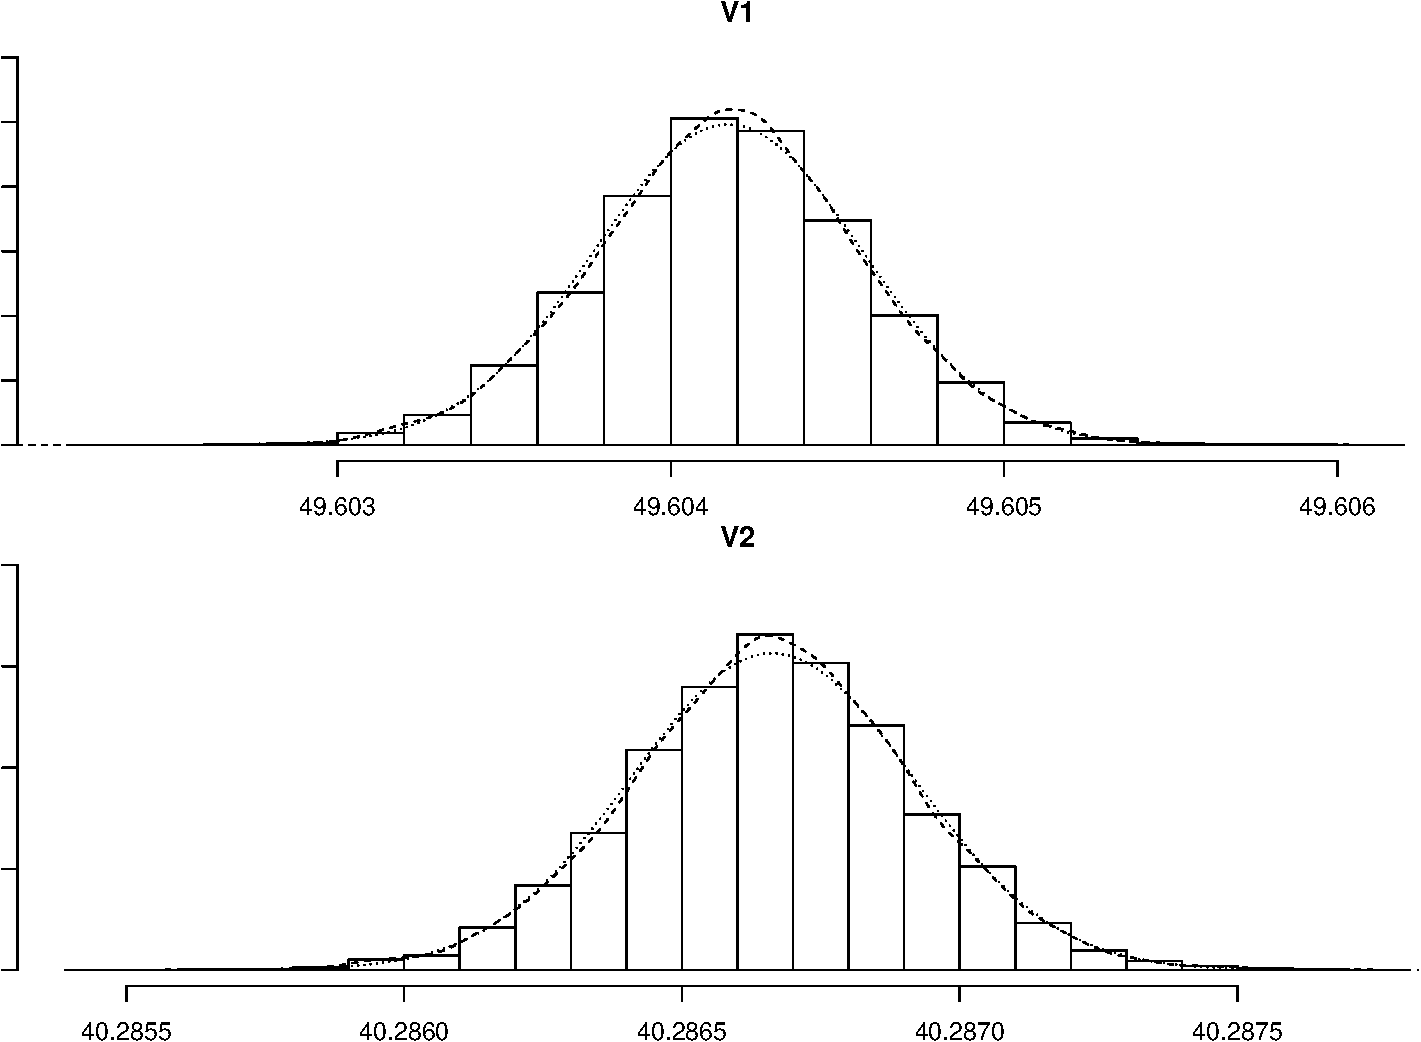
\includegraphics{est46114_s04_files/figure-beamer/visualizacion1-1.pdf}

\end{frame}

\begin{frame}{Visualizacion II}
\protect\hypertarget{visualizacion-ii}{}

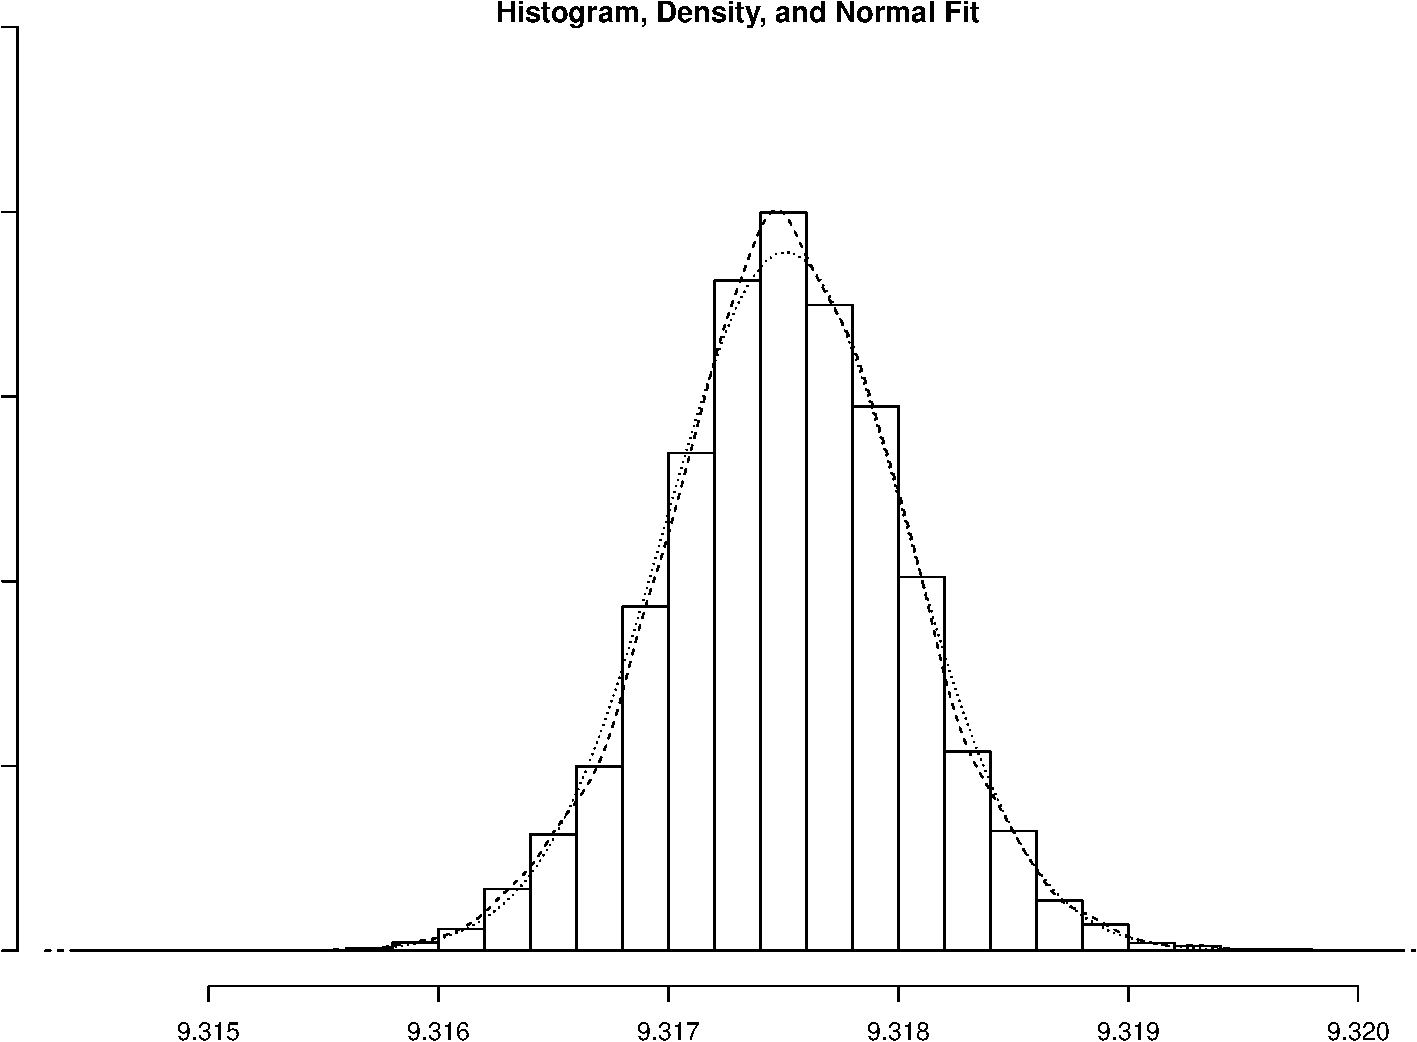
\includegraphics{est46114_s04_files/figure-beamer/visualizacion2-1.pdf}

\end{frame}

\begin{frame}[fragile]{Regla de decision (solucion lineal)}
\protect\hypertarget{regla-de-decision-solucion-lineal}{}

La par probabilidades para \(H_0\) y \(H_1\) (aproximadas por Monte
Carlo) son

\begin{Shaded}
\begin{Highlighting}[]
\NormalTok{prob_lin_h0 <-}\StringTok{ }\KeywordTok{length}\NormalTok{(}\KeywordTok{which}\NormalTok{(mu.sim}\FloatTok{.2}\NormalTok{[,}\DecValTok{1}\NormalTok{]}\OperatorTok{-}\NormalTok{mu.sim}\FloatTok{.2}\NormalTok{[,}\DecValTok{2}\NormalTok{] }\OperatorTok{>}\StringTok{ }\DecValTok{9}\NormalTok{))}\OperatorTok{/}\NormalTok{M}
\NormalTok{prob_lin_h0}
\end{Highlighting}
\end{Shaded}

\begin{verbatim}
## [1] 1
\end{verbatim}

y

\begin{Shaded}
\begin{Highlighting}[]
\NormalTok{prob_lin_h1 <-}\StringTok{ }\KeywordTok{length}\NormalTok{(}\KeywordTok{which}\NormalTok{(mu.sim}\FloatTok{.2}\NormalTok{[,}\DecValTok{1}\NormalTok{]}\OperatorTok{-}\NormalTok{mu.sim}\FloatTok{.2}\NormalTok{[,}\DecValTok{2}\NormalTok{] }\OperatorTok{<=}\StringTok{ }\DecValTok{9}\NormalTok{))}\OperatorTok{/}\NormalTok{M}
\NormalTok{prob_lin_h1}
\end{Highlighting}
\end{Shaded}

\begin{verbatim}
## [1] 0
\end{verbatim}

\textcolor{blue}{En este caso, la evidencia es contundente. {\bf Consideren que este NO es el caso, en general.}}

\end{frame}

\begin{frame}[fragile]{P1.b. Solucion lineal exacta}
\protect\hypertarget{p1.b.-solucion-lineal-exacta}{}

La solucion del problema, que hemos resulto via \texttt{simulacion} se
pudo haber obtenido analiticamente empleando el resultado de cerradura
bajo linealidad, considerando la aplicacion del vector \[
\boldsymbol{c}_{Hipotesis}=(0,1,0,0,-1,0),
\] a \[
\boldsymbol{\mu},
\] considernado que \[
(\boldsymbol{\mu},\boldsymbol{\Lambda}) \sim \text{N-Wi}(\boldsymbol{\mu},\boldsymbol{\Lambda}|\boldsymbol{m}_n,s_n,a_n,\boldsymbol{B}_n).
\]

\begin{itemize}
\item
  \textcolor{blue}{Se sigue que $\boldsymbol{c}_{Hipotesis}'\boldsymbol{\mu}$ sigue una distribucion $t$-univariada.}
\item
  \textcolor{red}{Los datos que simulamos, son una muestra `iid` de esta distribucion marginal.}
\item
  Solo problemas asociados con tranformaciones afines de
  \(\boldsymbol{X}\) o \(\boldsymbol{\mu}\) pueden resolverse de manera
  analitica cerrada. En general, sera util recurrir a herramientas de
  \texttt{simulacion\ estocastica}.
\end{itemize}

\end{frame}

\begin{frame}[fragile]{P2. Solucion no lineal}
\protect\hypertarget{p2.-solucion-no-lineal}{}

Ahora, la \texttt{solucion\ no\ lineal} a la pregunta
\textcolor{blue}{P2} puede plantearse como un problema de decision bajo
incertidumbre, considerando dos posibles hipotesis:

\textcolor{blue}{$H_0$: Hipotesis 0} \[
\mu_{Agriculture}/\mu_{Catholic} > 1.25.
\]

\textcolor{blue}{$H_1$: Hipotesis 1} \[
\mu_{Agriculture}/\mu_{Catholic} \leq 1.25.
\]

\end{frame}

\begin{frame}{Visualizacion III}
\protect\hypertarget{visualizacion-iii}{}

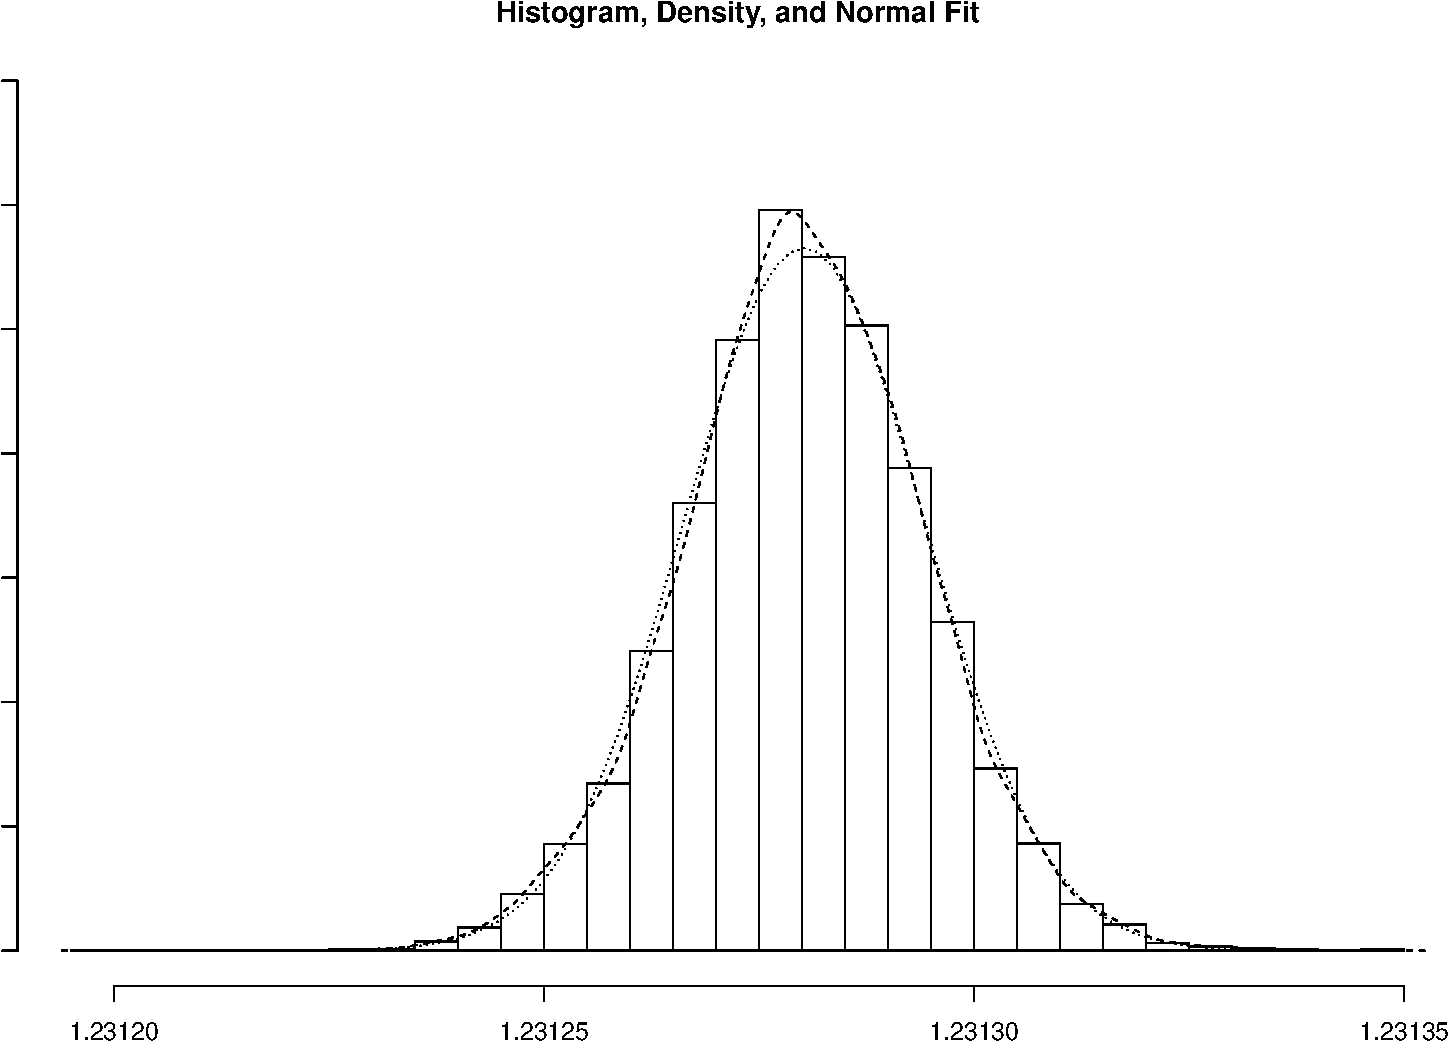
\includegraphics{est46114_s04_files/figure-beamer/visualizacion3-1.pdf}

\end{frame}

\begin{frame}[fragile]{Regla de decision (solucion lineal)}
\protect\hypertarget{regla-de-decision-solucion-lineal-1}{}

La par probabilidades para \(H_0\) y \(H_1\) (aproximadas por Monte
Carlo) son

\begin{Shaded}
\begin{Highlighting}[]
\NormalTok{prob_nolin_h0 <-}\StringTok{ }\KeywordTok{length}\NormalTok{(}\KeywordTok{which}\NormalTok{(mu.sim}\FloatTok{.2}\NormalTok{[,}\DecValTok{1}\NormalTok{]}\OperatorTok{/}\NormalTok{mu.sim}\FloatTok{.2}\NormalTok{[,}\DecValTok{2}\NormalTok{] }\OperatorTok{>}\StringTok{ }\FloatTok{1.25}\NormalTok{))}\OperatorTok{/}\NormalTok{M}
\NormalTok{prob_nolin_h0}
\end{Highlighting}
\end{Shaded}

\begin{verbatim}
## [1] 0
\end{verbatim}

y

\begin{Shaded}
\begin{Highlighting}[]
\NormalTok{prob_nolin_h1 <-}\StringTok{ }\KeywordTok{length}\NormalTok{(}\KeywordTok{which}\NormalTok{(mu.sim}\FloatTok{.2}\NormalTok{[,}\DecValTok{1}\NormalTok{]}\OperatorTok{/}\NormalTok{mu.sim}\FloatTok{.2}\NormalTok{[,}\DecValTok{2}\NormalTok{] }\OperatorTok{<=}\StringTok{ }\FloatTok{1.25}\NormalTok{))}\OperatorTok{/}\NormalTok{M}
\NormalTok{prob_nolin_h1}
\end{Highlighting}
\end{Shaded}

\begin{verbatim}
## [1] 1
\end{verbatim}

\textcolor{blue}{En este caso, la evidencia es contundente. {\bf Consideren que este NO es el caso, en general.}}

\end{frame}

\begin{frame}[fragile]{Ejercicio}
\protect\hypertarget{ejercicio}{}

Desarrollen las soluciones al problema \texttt{lineal} y
\texttt{no\ lineal} deferido ahora a las variables \[
X_{Agriculture}\text{ y }X_{Catholic},
\] en lugar de referirlo a
\(\mu_{Agriculture}\text{ y }\mu_{Catholic}\).

Desarrollen las soluciones via simulacion, considerando lo siguiente:
\begin{eqnarray}
\boldsymbol{\Lambda}|\text{datos} & \sim & \text{Wi}(\boldsymbol{\Lambda|a_n,\boldsymbol{B}_n}) \nonumber \\
\boldsymbol{\mu}|\boldsymbol{\Lambda},\text{datos} &\sim&\text{N}(\boldsymbol{\mu}|\boldsymbol{m}_n,s_n\boldsymbol{\Lambda}) \nonumber \\
\boldsymbol{X}|\boldsymbol{\mu},\boldsymbol{\Lambda},\text{datos} &\sim&\text{N}(\boldsymbol{x}|\boldsymbol{\mu},\boldsymbol{\Lambda}). \nonumber
\end{eqnarray}

\end{frame}

\begin{frame}{En la siguiente sesion}
\protect\hypertarget{en-la-siguiente-sesion}{}

Revisaremos como hacer:

\begin{enumerate}
\item
  Descomposion singular de matrices de covarianzas
\item
  Analisis de componentes principales
\item
  Analisis inferencial de componentes principales
\end{enumerate}

\end{frame}

\begin{frame}[fragile]{Lecturas complementarias}
\protect\hypertarget{lecturas-complementarias}{}

\begin{itemize}
\item
  Hothorn et al (2018) ``On multivariate t and Gauss probabilities in
  R''. \texttt{est46114\_s04\_suplemento1.pdf}
\item
  Martinez-Ovando (2016) ``Paradigma Bayesiano de Inferencia (Resumen de
  Teoria)'', \emph{Notas de clase EST-46114}.
  \textcolor{blue}{(De momento, no presten antencion a la descripcion de los metodos de simulacion transdimensionales.)}
  \texttt{est46114\_s03\_suplemento2.pdf}
\item
  Press (2005). ``Applied multivariate analysis, using Bayesian and
  frequentist methods of inference.'' Dover Pub.
  \textcolor{blue}{(Capitulo 4.)}
\end{itemize}

\end{frame}


\section[]{}
\frame{\small \frametitle{Table of Contents}
\tableofcontents}
\end{document}
